\paragraph{Western Bias in Wikidata}

Western bias analysis in Wikidata will be performed on 5 Wikidata classes: computer scientist, singer, memorial, university, and river. For each class, we collect the data for the western portion from 8 countries: Canada, France, Germany, Ireland, Poland, Switzerland, the United Kingdom (UK), and the United State of America (USA). For the non-western portion, we also selected 8 countries: China, Egypt, India, Indonesia, Japan, Morocco, Nigeria, and South Africa. The selected countries represent different continents to capture a diverse geographic distribution. Additionally, we focus on large and well-known countries to ensure the dataset is representative, as data from smaller countries may not provide meaningful insights due to limited coverage in Wikidata.

To analyze the bias, the first aspect that will be considered is the proportion of each regional category in every class. We assume that there are equal numbers of western and non-western and this will be the basis to determine if there is any bias in the data. Pearson's chi-square test (goodness-of-fit) is then performed to test the null and alternative hypotheses with significance level of \(\alpha=5\%\) as follows:

% \(H_0\): The proportions of western and non-western entities in a particular class are equal

% \(H_1\): The proportions of western and non-western entities in a particular class are not equal

\begin{table}[h]
    \centering
    \renewcommand{\arraystretch}{1.3}
    \begin{tabular}{|l p{12cm}|} 
        \hline
        \multicolumn{2}{|l|}{\textbf{Western Bias: Entity Count Gap (Pearson's chi-square test)}} \\
        \hline
        \textbf{$H_0$} & The proportions of western and non-western entities in a particular class are equal. \\
        \textbf{$H_1$} & The proportions of western and non-western entities in a particular class are not equal. \\
        \hline
    \end{tabular}
\end{table}

In terms of entity count, \autoref{tab:western - entity count} shows that there are big gaps between the westerners and non-westerners in all of the classes.

\begin{center}
\scriptsize
\begin{threeparttable}
\captionsetup{font=small}
\caption{Entity Count of 5 Wikidata Classes per Regional Category}
\label{tab:western - entity count}
\begin{tabular}{c | c c c c c c c} 

\toprule
    Class Name & Entity & Western & \CellWithForceBreak{Non- \\ western} & \%Western & \CellWithForceBreak{\%Non- \\ western}& $\chi^2$ & p-value \\ [0.5ex] 
\midrule
    Computer scientist & 6063 & 5446 & 617 & 0.90 & 0.10 & 3846.15 & 0.0 \\
    Singer & 43240 & 31039 & 12201 & 0.72 & 0.28 & 8206.99 & 0.0 \\
    Memorial & 4011 & 3836 & 175 & 0.96 & 0.04 & 3341.54 & 0.0 \\
    University & 6124 & 2398 & 3726 & 0.39 & 0.61 & 287.98 & 1.37e-64 \\
    River & 125567 & 70059 & 55508 & 0.56 & 0.44 & 1686.20 & 0.0 \\
    [1ex]
\bottomrule
\end{tabular}
\begin{tablenotes}
    \scriptsize
    \item{This table shows the entity count of 5 Wikidata classes per regional category. Chi-square test result shows the significance of difference between the entity count of the two genders male and female.}
\end{tablenotes}
\end{threeparttable}
\end{center}

From \autoref{tab:western - central tendency}, non-western entities generally have lower values of measure of central tendency (mean, median, mode). The range of property count of non-westerns is generally also lower than the westerns. Positive values of skewness (skewness > 0) and high kurtosis values (kurtosis > 3) in all classes denote the wealth distribution is right skewed and leptokurtic.

\begin{center}
\scriptsize
\begin{threeparttable}
\captionsetup{font=small}
\caption{Measures of Central Tendency of 5 Wikidata Classes per Regional Category}
\label{tab:western - central tendency}
\begin{tabular}{c | c c c} 
\toprule
    Class Name & \CellWithForceBreak{Mean \\ (o/w/n)} & \CellWithForceBreak{Median \\ (o/w/n)} & \CellWithForceBreak{Mode \\ (o/w/n)} \\ [0.5ex] 
\midrule
    Computer scientist & 35.00/35.87/27.24 & 29.00/29.00/22.00 & 21/15/16 \\
    Singer & 34.99/39.14/24.43 & 25.00/29.00/18.00 & 15/18/14 \\
    Memorial & 11.04/11.04/11.13 & 9.00/9.00/9.00 & 9/9/9 \\
    University & 23.11/31.61/17.63 & 17.50/24.00/16.00 & 6/6/6 \\
    River & 7.69/8.55/6.60 & 7.00/7.00/6.00 & 7/7/7 \\
    [1ex]
\bottomrule
\end{tabular}
\begin{tablenotes}
    \scriptsize
    \item{This table shows the measures of central tendency of 5 Wikidata classes per regional category. Each measure will have 3 values: o (overall), w (western), and n (non-western).}
\end{tablenotes}
\end{threeparttable}
\end{center}

\begin{center}
\scriptsize
\begin{threeparttable}
\captionsetup{font=small}
\caption{Measures of Dispersion and Symmetry of 5 Wikidata Classes per Gender Category}
\label{tab:western - dispersion and symmetry}
\begin{tabular}{c | c c c c c} 

\toprule
    Class Name & \CellWithForceBreak{Min \\ (o/w/n)} & \CellWithForceBreak{Max \\ (o/w/n)} & \CellWithForceBreak{Std. Deviation \\ (o/w/n)} & \CellWithForceBreak{Skewness \\ (o/w/n)} & \CellWithForceBreak{Kurtosis \\ (o/w/n)} \\ [0.5ex] 
\midrule
    Computer scientist & 4/4/5 & 441/441/145 & 25.15/25.67/18.15 & 3.02/3.02/2.37 & 20.90/20.83/8.49 \\
    Singer & 3/4/3 & 687/687/379 & 33.27/36.60/18.94 & 4.49/4.28/3.15 & 35.56/31.09/21.59 \\
    Memorial & 2/3/2 & 142/142/52 & 5.89/5.82/7.28 & 8.50/8.95/2.98 & 143.57/156.15/12.79 \\
    University & 2/2/2 & 234/234/166 & 20.00/25.88/12.25 & 2.37/1.65/2.22 & 10.34/5.33/12.70 \\
    River & 2/2/2 & 452/452/148 & 5.24/6.46/2.68 & 21.71/19.54/14.67 & 1152.84/868.56/465.42 \\
    [1ex]
\bottomrule
\end{tabular}
\begin{tablenotes}
    \scriptsize
    \item{This table shows the measures of dispersion and symmetry of 5 Wikidata classes per gender category. Each measure will have 3 values: o (overall), w (western), and n (non-western).}
\end{tablenotes}
\end{threeparttable}
\end{center}

Out of 5 classes, class of memorial is the only class where the null hypothesis is not rejected. In the other 4 classes, we can see a significant difference between the mean of the two reginal categories, which all are in favor of the western.

\begin{center}
\scriptsize
\begin{threeparttable}
\captionsetup{font=small}
\caption{F-Test, T-Test, and Welch's Test Result of 5 Wikidata Classes}
\label{tab:western - mean test}
\begin{tabular}{c | c c c c c c} 
\toprule
    Class Name & \CellWithForceBreak{F-Test \\ statistic} & \CellWithForceBreak{F-Test \\ p-value} & \CellWithForceBreak{T-Test \\ statistic} & \CellWithForceBreak{T-Test \\ p-value} & \CellWithForceBreak{Welch's Test \\ statistic} & \CellWithForceBreak{Welch's \\ p-value} \\ [0.5ex] 
\midrule
    Computer scientist & 2.00 & 1.00 & 8.13 & 5.10e-16 & 10.66 & 3.64e-25 \\
    Singer & 3.73 & 1.00 & 42.22 & 0.0 & 54.59 & 0.0 \\
    Memorial & 0.64 & 0.00 & -0.19 & 0.85 & -0.16 & 0.88 \\
    University & 4.46 & 1.00 & 28.40 & 8.23e-167 & 24.73 & 2.12e-123 \\
    River & 5.83 & 1.00 & 66.91 & 0.0 & 72.64 & 0.0 \\
 [1ex]
\bottomrule
\end{tabular}
\begin{tablenotes}
    \scriptsize
    \item{}
\end{tablenotes}
\end{threeparttable}
\end{center}

As with gender bias, measuring western bias in Wikidata cannot rely solely on entity counts. The number of entities associated with western and non-western regions may reflect real-world disparities in documentation or notability, making raw counts an unreliable indicator of bias. Similarly, measures of central tendency—such as the mean or median—fail to capture how representation is distributed across the full spectrum of prominence or wealth. To address these limitations, we apply the same metric introduced in the gender bias analysis: the relative expectation ratio. This measure compares a region’s share of entities within a given quantile to its expected share under equal representation. A ratio of 1 indicates proportional representation, while values above or below 1 signal overrepresentation or underrepresentation, respectively. This allows for a more nuanced, quantile-level understanding of how Western and non-Western entities are distributed in knowledge graphs like Wikidata.

\begin{table}[h]
    \centering
    \renewcommand{\arraystretch}{1.3}
    \begin{tabular}{|l p{12cm}|} 
        \hline
        \multicolumn{2}{|l|}{\textbf{Western Bias: Relative Expectation Ratios}} \\
        \hline
        \textbf{Insight 1:} & On average across all 5 classes, the less prominent segments are dominated by non-western entities, while the more prominent ones are dominated by western entities. The middle quantiles exhibit a zig-zag pattern, reflecting inconsistent representation between the two groups. \\
        \textbf{Insight 2:} & At the individual class level, 2 out of 5 classes display a particularly strong western dominance. The rests exhibit a zig-zag trend. \\
        \hline
    \end{tabular}
\end{table}

On average across all classes, the lower four quantiles (i.e., the less prominent or "poorer" segments) are predominantly composed of non-Western entities, while the top three quantiles (i.e., the more prominent or "wealthier" segments) are dominated by Western entities. The middle quantiles exhibit a zig-zag pattern, reflecting inconsistent representation between the two groups. At the individual class level, the computer scientist and singer classes display a particularly strong Western bias. In both classes, non-Western entities are consistently overrepresented in the lower quantiles (Q1–Q4), while Western entities are consistently overrepresented in the upper quantiles (Q5–Q6). This pattern suggests a clear stratification, with non-Western entities disproportionately concentrated in less prominent positions. The memorial, university, and river classes, however, deviate from this pattern and exhibit a zig-zag trend across quantiles. This suggests a more unstable distribution of Western and non-Western entities across the quantiles.

\begin{figure}
\centering 
\subfloat[Ratio of Class Wealth to Expectation per Cumulative Top Percentage - All Classes Average
\label{fig:test1 - western}]{%
  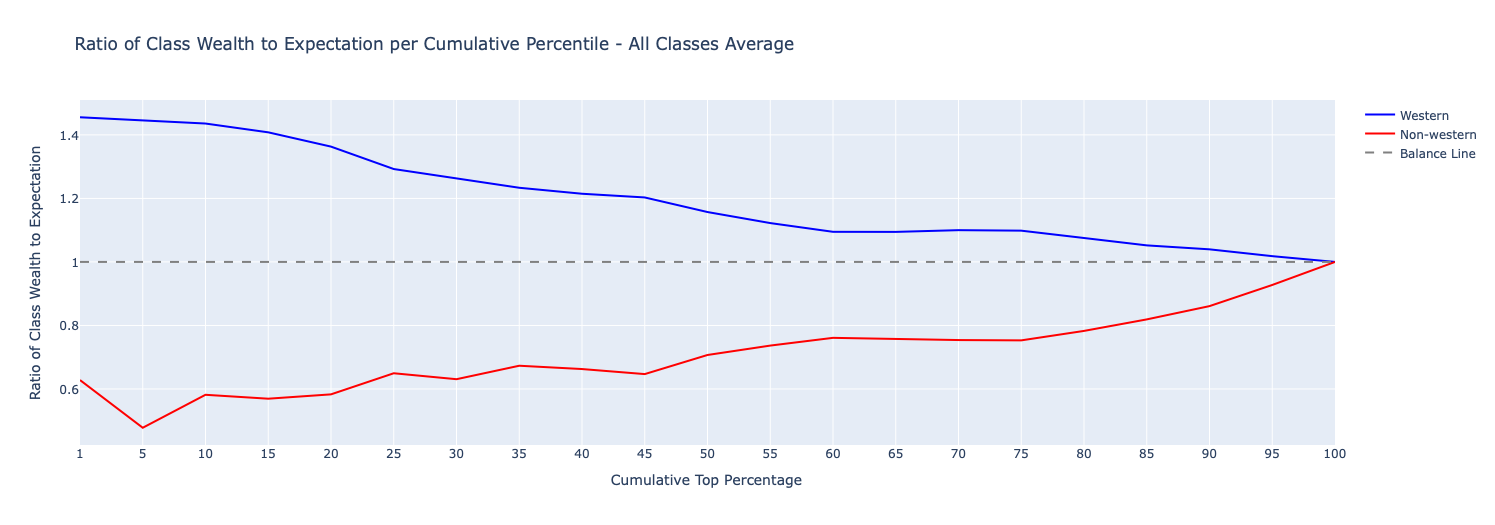
\includegraphics[clip,width=1.0\columnwidth]{Ratio of Class Wealth to Expectation per Cumulative Top Percentage - All Classes Average - Region}%
}

\subfloat[Ratio of Class Wealth to Expectation per Quantile - All Classes Average\label{fig:test2 - western}]{%
  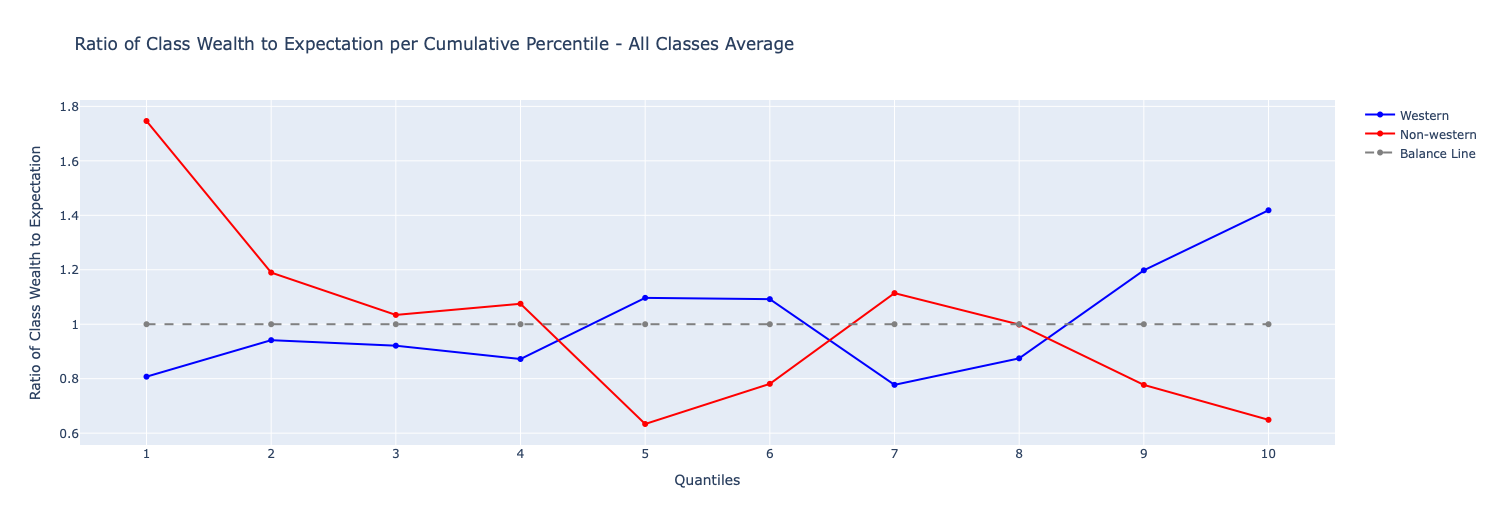
\includegraphics[clip,width=1.0\columnwidth]{Ratio of Class Wealth to Expectation per Quantile - All Classes Average - Gender - Region}%
}

\caption{Ratio of each regional wealth to expectaion}\label{fig:western - ratio of regional wealth to expectation}

\end{figure}